\documentclass[11pt]{article}
\setlength{\parindent}{0pt}
\setlength{\parskip}{0.5em}
\usepackage[a4paper, margin=2.7cm]{geometry}
\usepackage{graphicx}
\usepackage{float}

\begin{document}

\title{SDSD Assessed Coursework}
\author{Terence Tse : tt1611}
\maketitle
\newpage

\section{Graphical Design}
\begin{figure}[H]
\centering
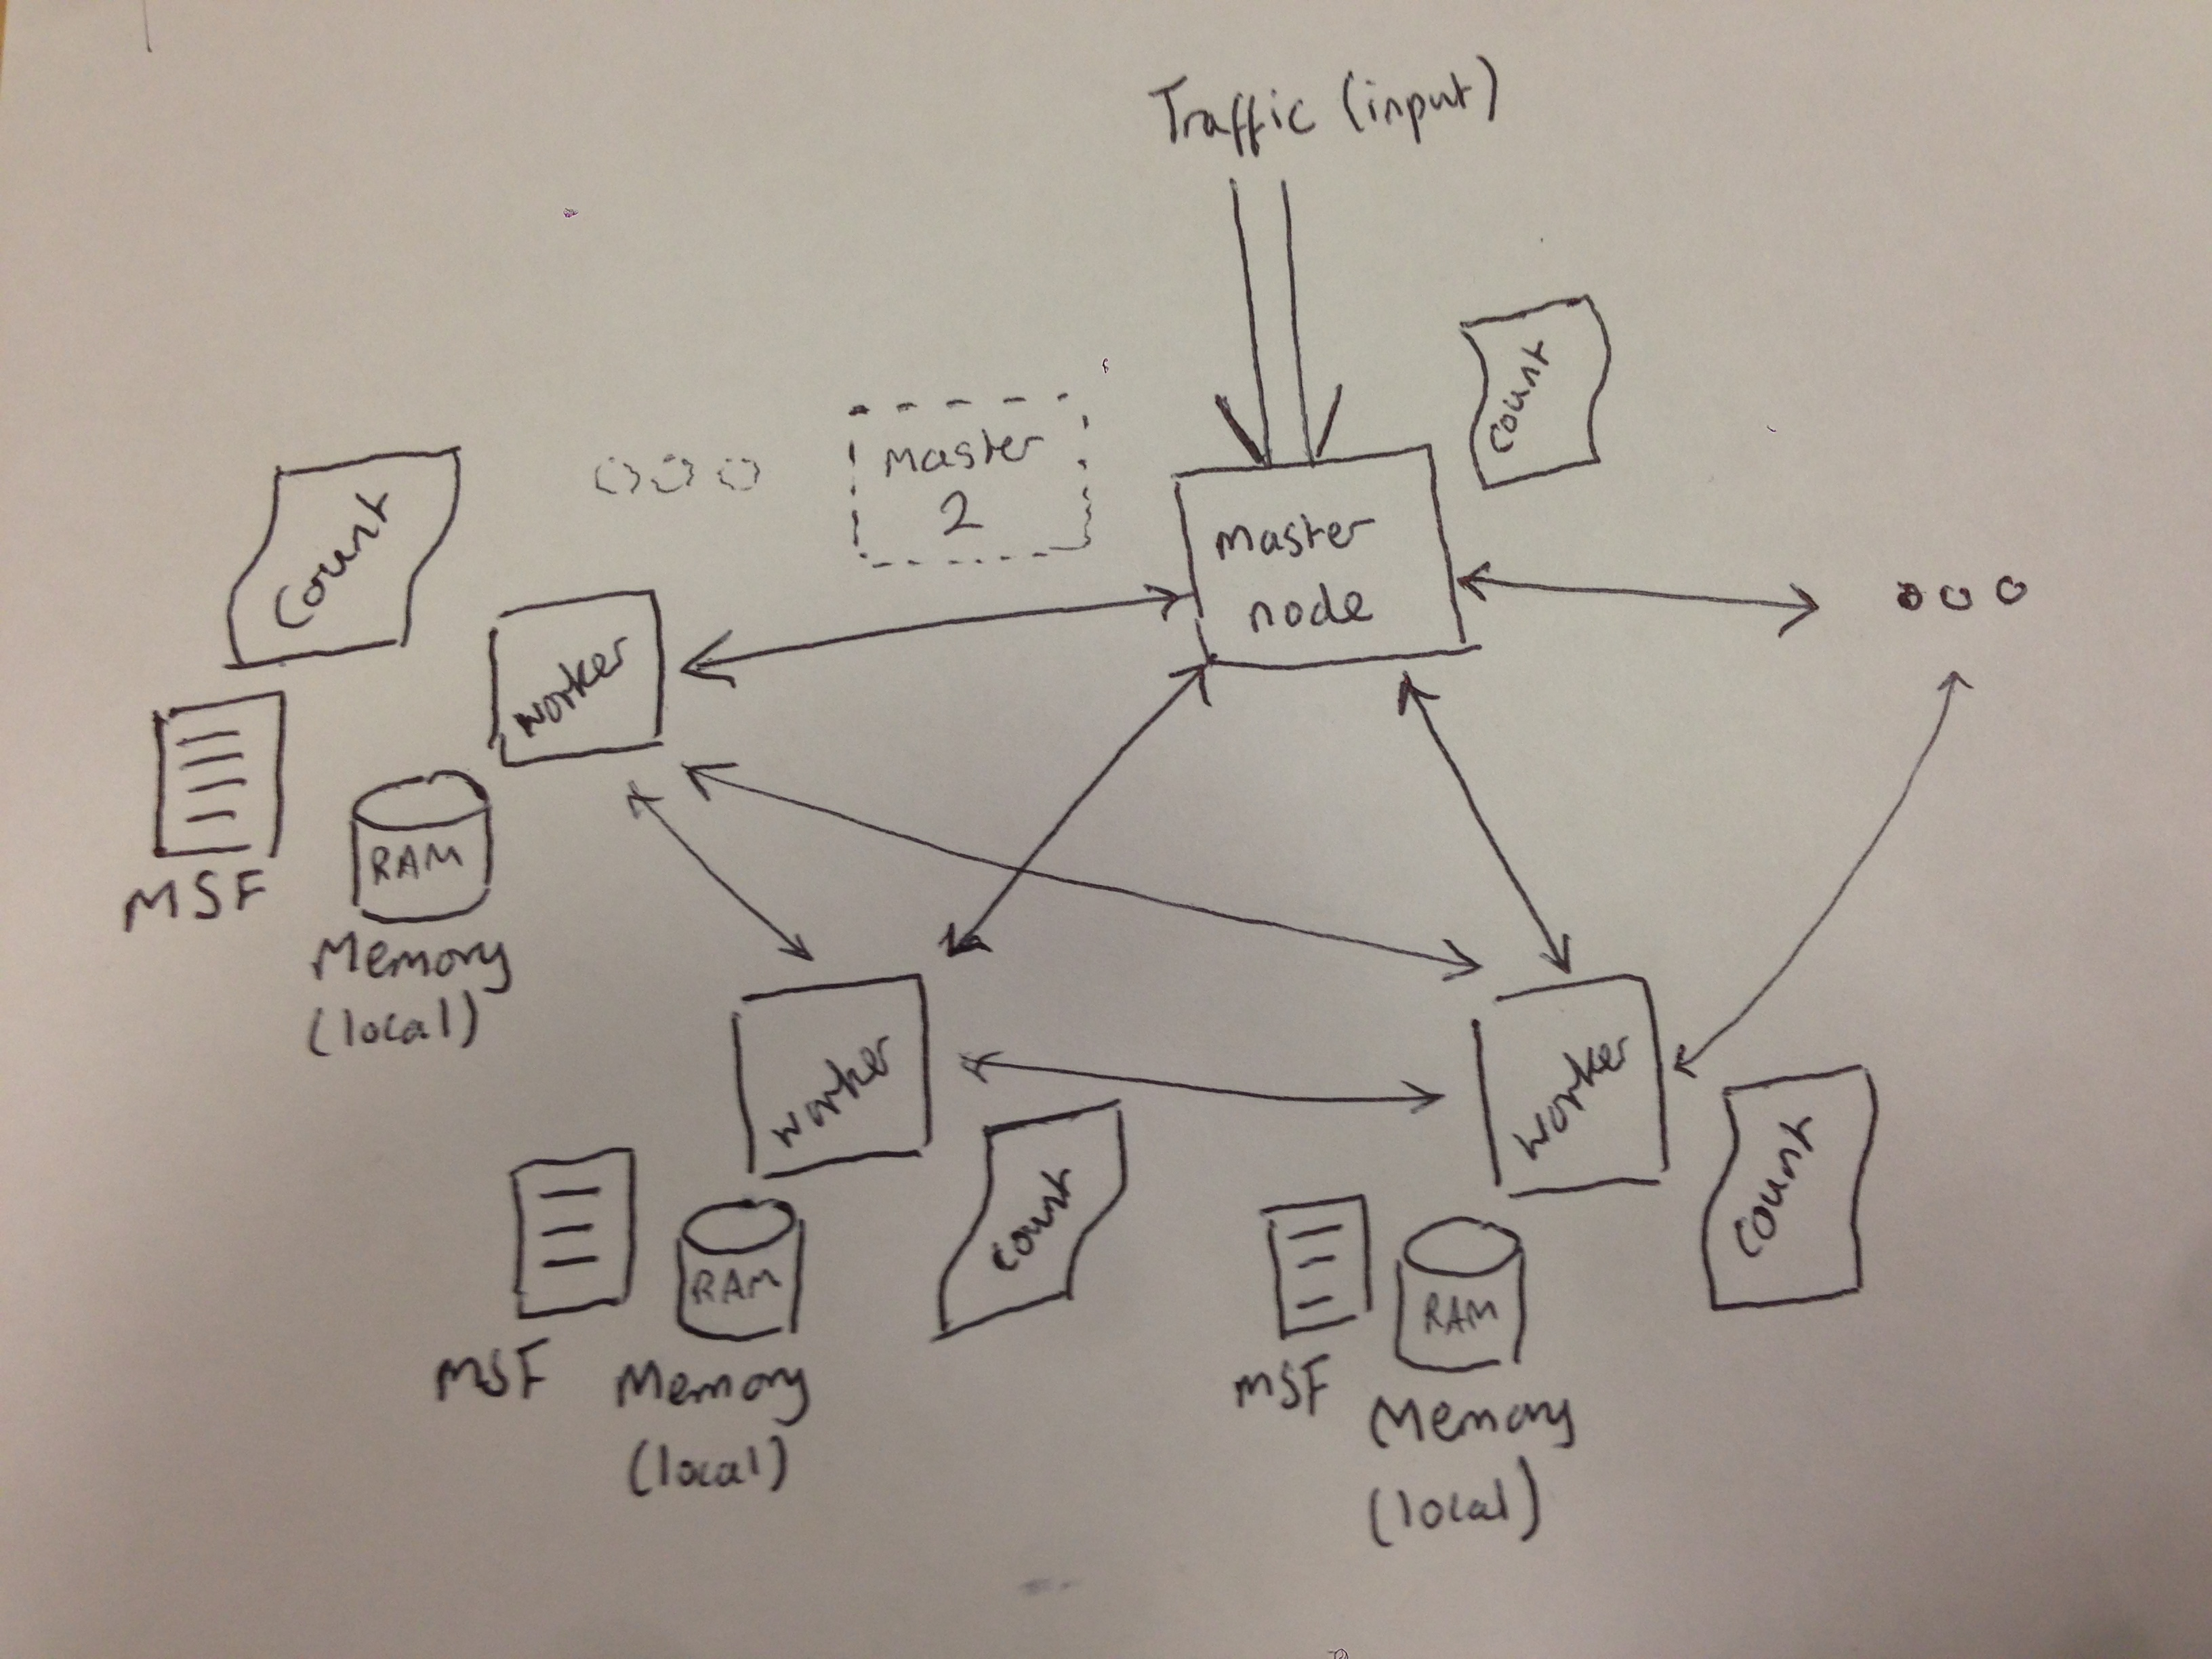
\includegraphics[scale=0.125]{pics/SDSD.jpg}
\end{figure}

\section{Description of Design}
In my design, I have a single centralised master node which
handles incoming network traffic. The node splits the
data into chunks which are sent to worker
nodes in a Map Reduce style except the data is sent with a task
in the style of the Resilient Distributed Datasets (RDD) model. This
will be done with a simple map function that performs an Identity 
function on a certain part of the data stream.

The worker nodes are other machines in the data centre. Each will
have a copy of the malicious signatures file (MSF) and store them in RAM.  
The worker will perform simple string matching against the 
malicious signatures, incrementing a local count of each within the
machine. These counts are stored as key value pairs, akin to map
reduce, with the malicious signatures being keys and
also being hashed. The hash function is the same across all the
machines in the data centre. The values are a SET of byte offsets
where the signatures start. The count of times the signatures were
seen is simply the length of this set and should contain no duplicates.

Some worker nodes are assigned the role of just reducing the incoming
data from other worker nodes, they will make up the reduce step which
will agglomerate the local counts of other work nodes to obtain the total
global count of seen malicious signatures on the master node for a certain
time point.

The master will then receive the returned work from the other 
nodes within the data centre(s) through reductions with maps,
filters and joins. The master also periodically sends the current
update count value of each malicious string to all the nodes
so that any can be queried and all return a consistent
value. (Master 2 mentioned later).

The workers and master can be queried for the current total(global) count of
malicious signatures detected as they all have a local copy.  To accommodate 
a "running" count, queried  workers can add their current counts to the 
locally saved global count. However this would cause differing reads 
depending on which worker is queried, although all of the reads are correct, 
they won't be consistent. As a result I think it's best to stick with 
returning the saved global count (same as master node). This preserves the 
Consistency property of CAP. Even if there is a network partitioning, if we 
consider failures, the Partitioning property is also held because each node
has a copy of the count and set of offsets.

\section{Design Assumptions and Considerations}
\begin{itemize}
\itemsep0em 
\item Although the system is essentially Map Reduce, we use RDDs because
we don't want processing to fall exponentially
behind input. As Map Reduce stores to disk, it won't do. 
We want to keep everything in RAM avoid I/O overheads.
\item Malicious signatures, although fixed-length are not all of
the same length.
\item The file containing the list of malicious
signatures the company checks for is small enough to be
stored in memory, not on disk.
\item Malicious signatures can be hashed and are such that there are no collisions.
\item The running total of malicious signatures detected must, at
every time, be correct and operates as an eventually correct 
system. The counts are guaranteed to be correct
or LESS than the actual amount of observed instances. 
\item Blissful ignorance of fault tolerant-design (system halts if node 
fails)extended to
communication as well, so all messages are guaranteed to reach their 
destinations.
\item Based on the CAP theorem, since we are choosing to 
tiptoe over Availability, the system created should be able
to satisfy the other two properties: Consistency and Partition.
\end{itemize}

\section{Parallelised work}
My design allows parallelised work as the network traffic is 
split into chunks (some of the the traffic is duplicated to 
account for possibilities of signatures lying across
chunks). The chunks are dealt with by the worker nodes in parallel. 
As a result, my design can allow parallelism up to a
certain degree which is bound by the size of the longest
malicious signature size. A chunk size of less than this would be sub 
optimal and require more comparisons across chunks which would
increase the duplication of the data and amount of work to be 
done.

\section{Scalability}
With a data centre of commodity machines, incremental, horizontal scaling 
should not be an issue. When the workload becomes larger, it
will be easy to add more machines, just like it is in Map Reduce. Since
these will all have RDDs on them, the computation is very fast and reduce 
steps can also be done quickly. A potential problem here is the
communication cost, as more workers get added to accommodate the
increasing traffic (from 100Gbps) , the communication 
overhead can increase as the system will only be as fast as its slowest 
link, more messages also have to be sent (containing global counts). 
However, having global counts makes querying the system fast and good if
the query is called often and machines are in data centres spread 
throughout the world. 

\section{Additional Considerations}
Though I outlined earlier my design assumptions and considerations, 
I would like to address some of them here. 
\begin{itemize}
\item Since we are using RDDs, the system is already quite fault tolerant
due to the nature of its bulk writes.
\item In addition, RDD is good for coarse grained transforms, which is
what we will be doing to the input data, we are simply taking some part
of the incoming traffic. 
\item Using the RDD model will allow the running of back up copies of slow 
tasks just like Map Reduce to reduce the impact of stragglers.
\item As a result, even if the memory is only large enough to hold the MSF
in my design, this method will only be as slow as Map Reduce due to spilling 
over into disk.
\item If there is a failure by a worker node, all that has to be done is
to rerun the same task given to that worker upon recovery or upon another
node.
\item MASTER 2 in my diagram is there to account for the case where we 
consider fault tolerance and failures in the network. This design could
be extended further to include several masters (not limited to 2) which 
receive chunked parts
of input and then are in charge of their own mini-clusters. Each will 
receive the global count at the end, just like the central master right now.
In my original design, the one point of failure would be the centralised
master. If that goes down the whole thing stops. However, using RDDs, we may
be able to reconstruct data due to stroing lineage. Having multiple
master nodes will increase the chance of failure but there will be another
master that can take up the failed master's job and be in charge of its
cluster until it recovers (if it does). Since all the masters will have a 
global count and set of offsets, they can continue operations and just 
continue adding to and incrementing this. 
\item I was very unsure about the byte offsets and how these would be 
stored. I was considering using some method of splitting the data based on
time and using time stamps. Thus, using a combination of timestamp and 
offset, it would be possibly easier to store offsets rather than saving
large exponents and mantissas. However this would require some kind of 
global clock to synchronise in the case of multiple master nodes. As we
know, this would be quite difficult in a distributed system and may 
require vector clocks or Google's TrueTime. If
there was one master, then the time splitting should be consistent.
 
\end{itemize}

\end{document}